\documentclass[a4paper]{article}
\setlength{\parskip}{11pt plus 1pt minus 1pt}

% prutsen met fonts, xeLaTeX compiler nodig!
%\usepackage{fontspec}
%\setmainfont{[HumorSans.ttf]}

%% Language and font encodings
\usepackage[dutch]{babel}
\usepackage[utf8]{inputenc}
\usepackage[T1]{fontenc} 
\usepackage[backend=bibtex]{biblatex}
\usepackage{url}
\addbibresource{bibliografie.bib}


%% Sets page size and margins
\usepackage[a4paper,top=3cm,bottom=2cm,left=1in]{geometry}

%% Useful packages
\usepackage{amsmath}
\usepackage{graphicx}
\usepackage[colorinlistoftodos]{todonotes}
\usepackage[colorlinks=true, allcolors=blue]{hyperref}
\usepackage{booktabs}
\usepackage{float}
\usepackage{siunitx}
%\usepackage[backend=biber,style=authortitle-comp]{biblatex}


\title{Gedwongen oscillatie en resonantie}
\author{Pieter Luyten \& Alex Windey }
\date{December 2018}

\begin{document}

\maketitle

\section{Inleiding}
In dit practicum worden de fenomenen van mechanische gedempte oscillatie en resonantie bestudeerd. (mms nog is brak bij)

\section{Materiaal \& Methoden}
In dit practicum wordt gebruik gemaakt van een gedempte harmonische oscillator met een gedwongen sinusoïdale aandrijving. Hierbij is de harmonische oscillator een massa-veersysteem en wordt de aandrijving gecreëerd door een motor. In dit geval oscilleert de massa onder water waardoor er ook demping optreedt. Het toepassen van de tweede wet van Newton op dit massa-veersysteem geeft volgende formule:
\begin{equation}
    m\frac{d^2x}{dt^2} = -kx -\eta \frac{dx}{dt} + F_0 e^{i\omega t}
\label{eq: 2e wet}
\end{equation}
\\
Hierin is $m$ de massa in $[kg]$, $k$ $[N/m]$de veerconstante en $x$ de uitwijking van de massa t.o.v. de evenwichtspositie in $[m]$. De demingskracht wordt evenredig met de snelheid genomen, waarbij $\eta$ $[N (m/s)^{-1}]$ de dempingscoëfficient is. De sinusoïdale aandrijvingskracht wordt geschreven als $F_0 e^{i\omega t}$ zodat $F_0$ $[N]$ de amplitude van de beweging is, $\omega$ $[Hz]$ de frequentie en $t$ $[s]$ de tijd. Oplossen van differentiaalvergelijking \ref{eq: 2e wet} naar $x$ geeft:
\begin{equation}
    x = \frac{F_0}{m\left( \sqrt{(\omega_0^2 - \omega^2)^2 + (\omega\frac{\eta}{m})^2} \right)} e^{i \omega t + i\phi (\omega) }
\label{eq: oplossing}    
\end{equation}
met
\begin{equation}
    \phi = - \operatorname{Bgtan}{\left (\frac{\eta \omega}{m \left(- \omega^{2} + \omega_{0}^{2}\right)} \right )}
    \label{eq:phi}
\end{equation}
\\
In vergelijking \ref{eq: oplossing} is de eigenfrequentie van het massa-veersysteem $\omega_0 = \sqrt{\frac{k}{m}}$ en $\phi(\omega)$ het faseverschil t.o.v. de aandrijving. De absolute waarde nemen van de oplossing voor $x$ geeft de amplitude $A [m]$ van de oscillatie:
\begin{equation}
    A = \frac{F_{0}}{m \sqrt{\frac{\eta^{2} \omega^{2}}{m^{2}} + \left(- \omega^{2} + \omega_{0}^{2}\right)^{2}}}
    \label{eq:A}
\end{equation}
Deze formules worden gebruikt door om de data van de experimenten te fitten. Om het faseverschil te kunnen fitten is er echter nog wat manipulatie van de data of de vergelijking nodig. De meetopstelling gebruikt namelijk een andere conventie voor het teken van de faseverschuiving dan die in vergelijking \ref{eq:phi}. Ook hangt de waarde van het fasevershil af van de beginpositie van de aandrijving, dit zorgt voor een verschuiving met een constante van de fase. om te kunnen fitten wordt concreet het teken van het rechterlid van vergelijking \ref{eq:phi} gewisseld en wordt er een extra, constante, term $\phi_0 [rad]$ bij opgeteld. Dit geeft volgende vergelijking om te fitten:
\begin{equation}
    \phi = \operatorname{Bgtan}{\left (\frac{\eta \omega}{m \left(- \omega^{2} + \omega_{0}^{2}\right)} \right )} + \phi_0
    \label{eq:fit_phi}
\end{equation}
\\
Formules \ref{eq:A} en \ref{eq:phi} voor de amplitude en het faseverschil kunnen herschreven worden in termen van $X = \frac{F_0}{k}$, een dimensieloze frequentie $w = \frac{\omega}{\omega_0}$ en een dimensieloze $b = \frac{\eta}{\sqrt{2km}}$.
De bekomen dimensieloze formule voor de amplitude $A$ is dan:
\begin{equation}
    A = \frac{X}{\sqrt{2 b^{2} w^{2} + \left(w^{2} - 1\right)^{2}}}
    \label{eq:A_dim}
\end{equation}

Ook het faseverschil kan dan in een dimensieloze vorm geschreven worden:
\begin{equation}
    \phi = - \operatorname{Bgtan}{\left (\frac{\sqrt{2} b w}{- w^{2} + 1} \right )}
    \label{eq:phi_dim}
\end{equation}
\\
In Figuur \ref{fig:A_dim} wordt de amplitude $A$ in functie van de dimensieloze frequentie $w$ voor verschillende dempingssterktes $b$ geplot.

\begin{figure}[h]
    \centering
    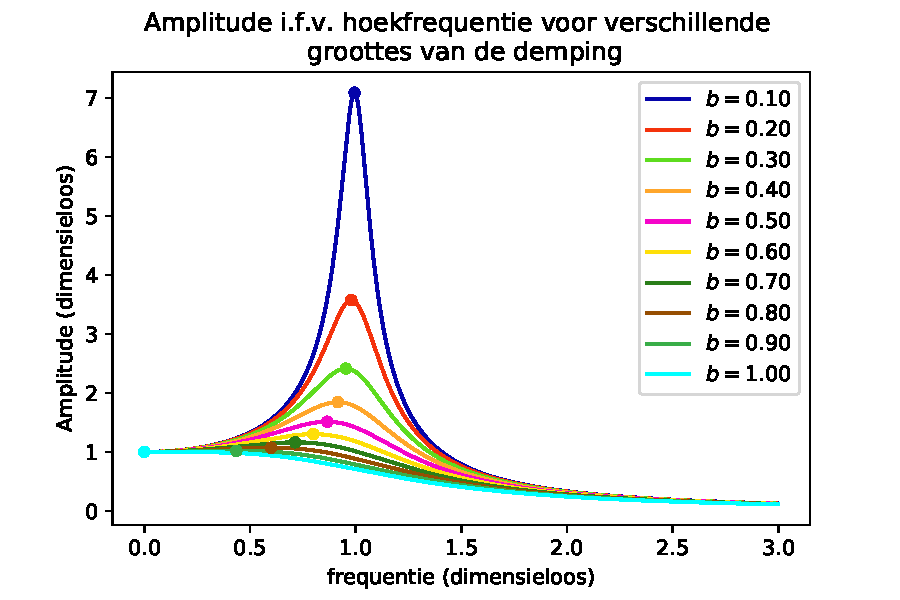
\includegraphics[width=0.8\linewidth]{dimensieloze_amplitude.pdf}
    \caption{De amplitude in functie van de hoekfrequentie voor de dimensiloze eenheden}
    \label{fig:A_dim}
\end{figure}

\begin{figure}
    \centering
    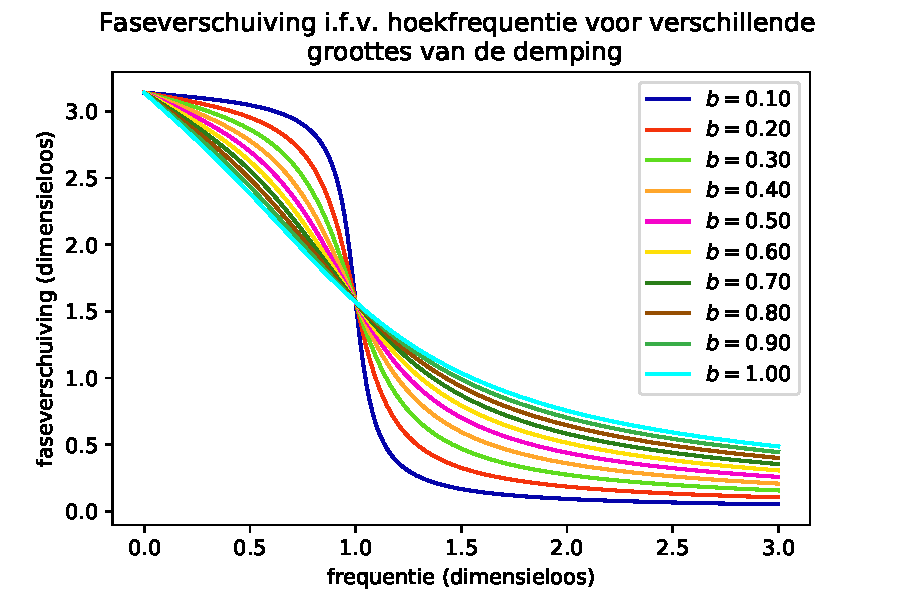
\includegraphics[width=0.8\linewidth]{dimensieloze_faseverschuiving.pdf}
    \caption{De faseverschuiving in functie van een dimensieloze hoekfrequentie $w$ voor een aantal waardes van de dimensieloze dempingsfactor $b$. De geplotte functie is vergelijking \ref{eq:phi_dim}}
    \label{fig:my_label}
\end{figure}



De gebruikte meetopstelling wordt weergegeven in Figuur \ref{fig: meetopstelling}. 

\begin{figure}[H]
  \centering
    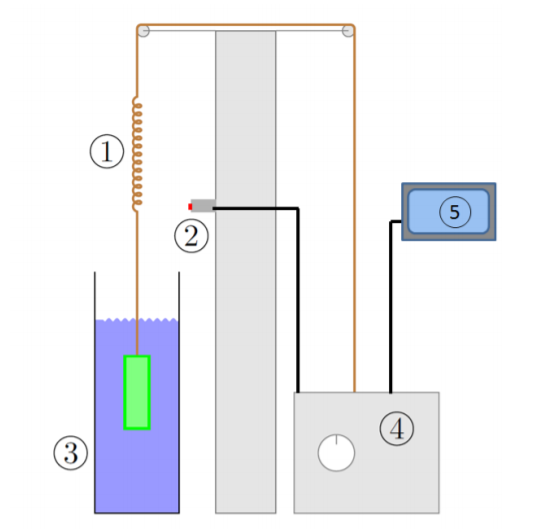
\includegraphics[width=0.5\textwidth]{Capture}
    \caption{Schema van de meetopstelling}
  \label{fig: meetopstelling}
\end{figure}


\section{Resultaten}

\begin{table}[h]
    \centering
    \begin{tabular}{|c|c|c|c|c|c|}
        \toprule
        Reeks & $ \omega_0 [rad/s] $ & $ m [kg] $ & $ \eta [N / (m/s)] $ & $ F_0 [N] $ & $\phi_0 [rad]$\\
        \midrule
        amplitude & $ 11.342 \pm 0.010 $ & $ 12.3 \pm 0.3 $ & $ 8.35 \pm 0.13 $ & $ 8.70 \pm -0.10 $ & \\
        fase & $11.301 \pm 0.010$& $7.3 \pm 0.5$& $3.4 \pm 0.2$& &$-0.144 \pm 0.016$\\
        \bottomrule
    \end{tabular}
    \caption{De gefitte parameters voor de data van het experiment met een kleine demping. De waardes in een rij komen overeen met de fit door de data in de kolom reeks, dus met de fit van amplitude i.f.v. de hoekfrequentie of van de fase i.f.v. de hoekfrequentie.}
    \label{tab:params_klein}
\end{table}

\begin{figure}[h]
\centering
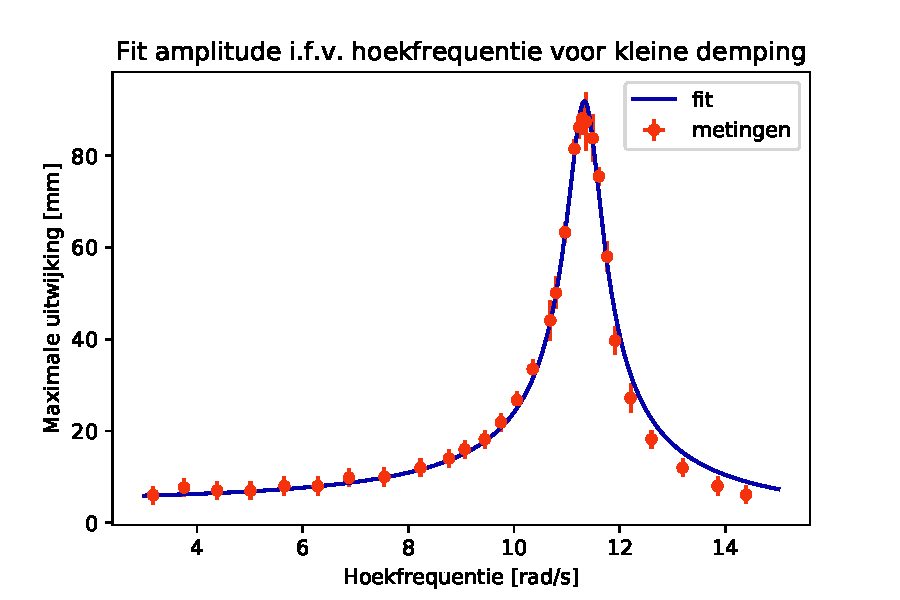
\includegraphics[width=0.8\linewidth]{fit_amplitude_klein.pdf}
\caption{De gemeten amplitudes in functie van de hoekfrequentie met kleine demping en de fit door de data. De gefitte functie is vergelijking \ref{eq:A}, de fitparameters staan in tabel \ref{tab:params_klein} in de rij amplitude.}
\end{figure}

\begin{figure}[h]
\centering
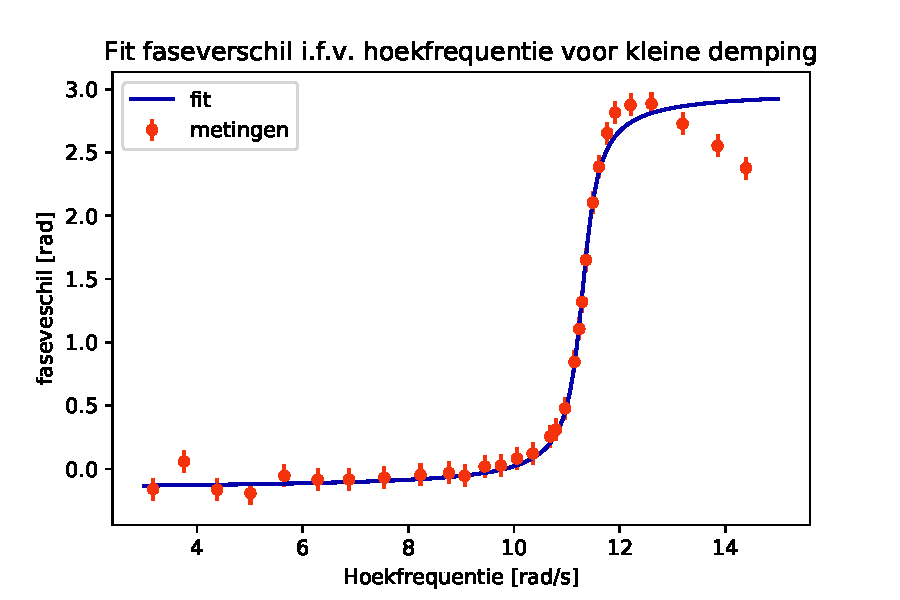
\includegraphics[width=0.8\linewidth]{fit_fase_klein.pdf}
\caption{De gemeten faseverschillen in functie van de hoekfrequentie met kleine demping en de fit door de data. De gefitte functie is vergelijking \ref{eq:fit_phi}, de fitparameters staan in tabel \ref{tab:params_klein} in de rij fase.}
\end{figure}

\begin{table}[h]
    \centering
    \begin{tabular}{|c|c|c|c|c|c|}
        \toprule
        Reeks & $ \omega_0 [rad/s] $ & $ m [kg] $ & $ \eta [N / (m/s)] $ & $ F_0 [N] $ & $\phi_0 [rad]$\\
        \midrule
        amplitude & $ 10.88 \pm 0.02 $ & $ 2.81 \pm 0.02 $ & $ 15.72 \pm 0.08 $ & $ 10.24 \pm 0.04 $ & \\
        fase & $10.61 \pm 0.03$& $2.70 \pm 0.06$& $11.7 \pm 0.2$ & & $-0.259 \pm 0.008$\\
        \bottomrule
    \end{tabular}
    \caption{De gefitte parameters voor de data van het experiment met een grote demping. De waardes in een rij komen overeen met de fit door de data in de kolom reeks, dus met de fit van amplitude i.f.v. de hoekfrequentie of van de fase i.f.v. de hoekfrequentie.}
    \label{tab:params_groot}
\end{table}

\begin{figure}[h]
\centering
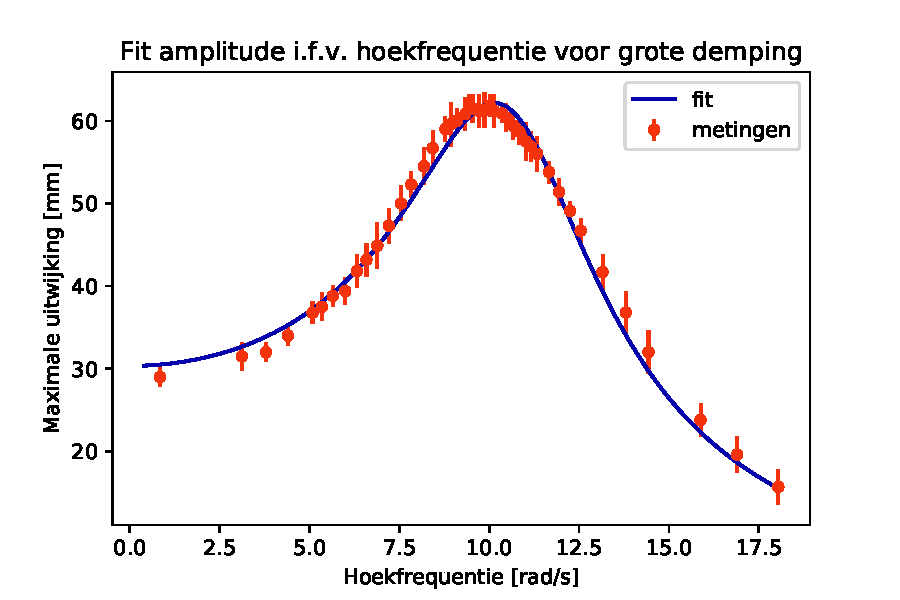
\includegraphics[width=0.8\linewidth]{fit_amplitude_groot.pdf}
\caption{De gemeten amplitudes in functie van de hoekfrequentie met grote demping en de fit door de datapunten. De gefitte functie is vergelijking \ref{eq:A}, de fitparameters staan in tabel \ref{tab:params_groot} in de rij amplitude.}
\end{figure}

\begin{figure}[h]
\centering
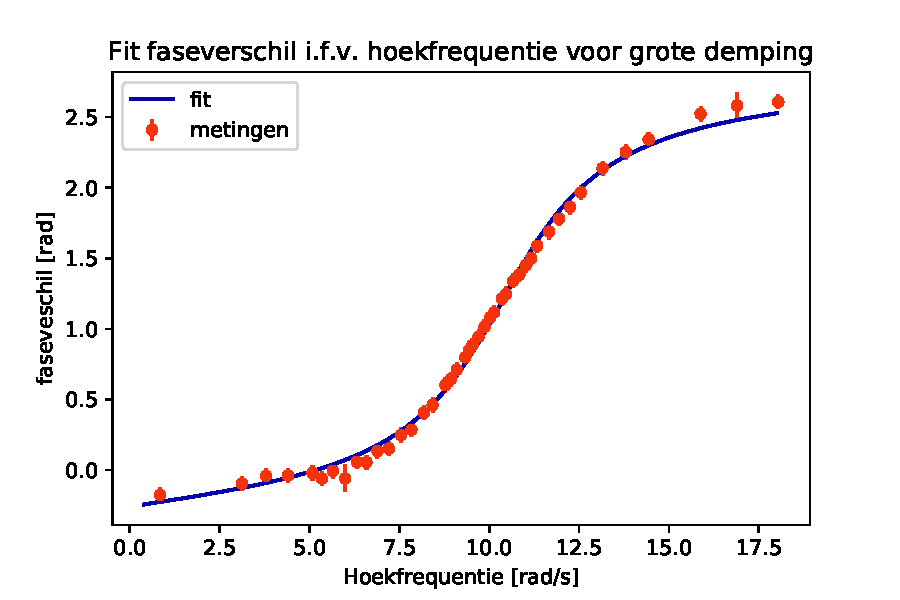
\includegraphics[width=0.8\linewidth]{fit_fase_groot.pdf}
\caption{De gemeten faseverschillen in functie van de hoekfrequentie met grote demping en de fit door de datapunten. De gefitte functie is vergelijking \ref{eq:fit_phi}, de fitparameters staan in tabel \ref{tab:params_groot} in de rij fase.}
\end{figure}

\end{document}
